% The main file for my thesis
% each \textbf{chapter} is included from this main file
\documentclass[11pt,a4paper]{uolthesis}
%\documentclass[11pt,a4paper]{article}
%\usepackage{alltt,float}
%\usepackage{lgrind}
\usepackage{url}                    % for better handling of URL
\usepackage{lscape}                 % allow to use \begin{landscape}, which makes a page in landscape.
%\usepackage{subfigure}
\usepackage{mathrsfs}
\usepackage{graphicx}
%\usepackage{caption2}
\usepackage{epstopdf}
\usepackage{apacite}
\usepackage{natbib}
\usepackage{amsmath}
\usepackage{tikz}
\usepackage{pgfplots}
\usepackage{caption}
\usepackage{subcaption}
\usepackage{pgfgantt}
\usepackage{multirow}

\usetikzlibrary{shapes.arrows}

\newcommand{\citepos}[1]{\citeauthor{#1}'s \citeyearpar{#1}}
\newcommand{\citeposs}[1]{\citeauthor{#1}' \citeyearpar{#1}}

%Modify the Figure Captionequ1-1:shannon
%\renewcommand{\figurename}{Fig.}
%set the figures captions
%\captionstyle{hang} \setcaptionwidth{13cm}
%**********************************************

% correct bad hyphenation here
\hyphenation{op-tical}
% use less hyphenation
\lesshyphenation
% or totally stop it
%\nohyphenation

% include them only, as I am currently working on them
%\includeonly{ch1/ch1}

% begin the main document
\begin{document}

% include the title pages, acknowledgements, and author's publications

\title{A Geometric Method for Context Sensitive Distributional Semantics}

\author{Stephen McGregor}
\department{School of Electronic Engineering and Computer Science} \college{Queen Mary, University of London}
\degree{Doctor of Philosophy} \degreemonth{September} \degreeyear{2017}

%% By default, the thesis will be copyrighted to MIT.  If you need to
%% copyright the thesis to yourself, just specify the `vi' documentstyle
%% option.  If for some reason you want to exactly specify the copyright
%% notice text, you can use the \copyrightnoticetext command.
%\copyrightnoticetext{\copyright ~University of London, 2006}

% The dedication info.
%\dedication{TO MY FAMILY}

% Make the titlepage based on the above information.  If you need something
% special and can't use the standard form, you can specify the exact text of
% the titlepage yourself.  Put it in a titlepage environment and leave blank
% lines where you want vertical space. The spaces will be adjusted to fill
% the entire page. The dotted lines for the signatures are made with the
% \signature command.

% Make the first title page
\maketitle

% make the dedication page
%\makededication

\makedeclaration

% Start to count page number from abstract page
\pagestyle{plain}%
\setcounter{page}{1}
\pagenumbering{roman} %

% The abstractpage environment sets up everything on the page except the
% text itself.
%
% You can either \input (*not* \include) your abstract file, or you can put
% the text of the abstract directly between the \begin{abstract} and
% \end{abstract} commands.
\begin{abstract}
%\input{abstract}
% abstract goes here
This thesis describes a novel methodology, grounded in the distributional semantic paradigm, for building context sensitive models of word meaning, affording an empirical exploration of the relationship between words and concepts. Anchored in theoretical linguistic insight regarding the contextually specified nature of lexical semantics, the work presented here explores a range of techniques for the selection of subspaces of word co-occurrence dimensions based on a statistical analysis of input terms as observed within large-scale textual corpora. The relationships between word-vectors that emerge in the projected subspaces can be analysed in terms of a mapping between their geometric features and their semantic properties. The power of this modelling technique is its ability to generate ad hoc semantic relationships in response to an extemporaneous linguistic or conceptual situation. 

The product of this approach is a generalisable computational linguistic methodology, capable of taking input in various forms, including word groupings and sentential context, and dynamically generating output from a broad base model of word co-occurrence data.  To demonstrate the versatility of the method, this thesis will present competitive empirical results on a range of established natural language tasks including word similarity and relatedness, metaphor and metonymy detection, and analogy completion. A range of techniques will be applied in order to explore the ways in which different aspects of projected geometries can be mapped to different semantic relationships, allowing for the discovery of a range of lexical and conceptual properties for any given input and providing a basis for an empirical exploration of distinctions between the semantic phenomena under analysis. The case made here is that the flexibility of these models and their ability to extend output to evaluations of unattested linguistic relationships constitutes the groundwork for a method for the extrapolation of dynamic conceptual relationships from large-scale textual corpora. 

This method is presented as a complement and a counterpoint to established distributional methods for generating lexically productive word-vectors. Where contemporary vector space models of distributional semantics have almost universally involved either the factorisation of co-occurrence matrices or the incremental learning of abstract representations using neural networks, the approach described in this thesis preserves the connection between the individual dimensions of word-vectors and statistics pertaining to observations in a textual corpus. The hypothesis tested here is that the maintenance of actual, interpretable information about underlying linguistic data allows for the contextual selection of non-normalised subspaces with more nuanced geometric features. In addition to presenting competitive results for various computational linguistic targets, the thesis will suggest that the transparency of its representations indicates scope for the application of this model to various real-world problems where an interpretable relationship betweendata and output is highly desirable. This, finally, demonstrates a way towards the productive application of the theory and philosophy of language to computational linguistic practice.

\end{abstract}

% Acknowledgments
%
% You can either \input (*not* \include) your acknowledgments file, or you can put
% the text of the acknowledgments directly between the \begin{acknowledgments} and
% \end{acknowledgments} commands.
%\begin{acknowledgments}
%\input{acknowledgments}
%Acknowledgment goes here...

%\end{acknowledgments}

%\begin{context}
%The term \emph{context} has been used widely and variously by authors in both theoretical and computational linguistics, and with good reason, as various sense of the concept of context are clearly at play in any serious discussion of the interplay between language and cognition.  Statistically minded computational linguists in particular, of whom I would like to count myself as one, have often used \emph{context} to refer to the window of co-occurrence in which a word token is observed within a sample of text.  In his description of a co-occurrence statistic for measuring semantic similarity, \cite{Salton1992b} introduced the term \emph{context space} to refer to a space of co-occurrence dimensions, a terminology subsequently adopted by \cite{BurgessEA1997} in relation to their HAL system.  This notion of proximity within a text as context has persevered in the natural language processing literature.

%Theoretical linguists and cognitive scientists, on the other hand, have tended to treat \emph{context} as a thing 

%So 

%and this nomenclature has been carried on by subsequent researchers interested in the idea that cognition, conceptualisation, and, correspondingly, language are always in some way specified by a situation in the world.

%In this thesis, I will endeavour to use the term \emph{context} strictly in reference to the latter notion of 

%\end{context}

\begin{glossary}
\begin{description}
\item[base space] A high dimensional, sparse vector space of word-vectors, delineated in terms of dimensions of co-occurrence statistics.
\item[context] The situation -- environmental, cognitive, perceptual, linguistic, and otherwise -- in which an agent finds itself and applies language to meaning.
\item[contextual input] A set of words characteristic of a conceptual category or semantic relationship used to generate a subspace for the modelling of semantic phenomena.
\item[dimension selection] The process of contextually choosing a subset of dimensions in order to project a subspace from a base space.
\item[co-occurrence] The observation of one word in proximity to another in a corpus.
\item[co-occurrence statistic] A measure of the tendency for one word to be observed in proximity to another across a corpus.
\item[co-occurrence window] The boundary defining the proximity within which two words are considered to be co-occurring, typically a distance in terms of words within a sentence.
\item[methodology] The process of building base spaces from observations of co-occurrences within a corpus and contextually projecting subspaces through dimension selection.
\item[model] An application of methodology to a particular linguistic task or experiment, sometimes including task specific statistical analysis techniques.
\item [subspace] A context specific lower-dimensional projection from a base space, effectively mapping semantic relationships to a context by way of the geometric relationships between word-vectors.
\item[word-vector] A high-dimensional geometrically situated semantic representation of a word, constructed as an array of co-occurrence statistics.
\end{description}
\end{glossary}


%\include{format}
% Generate table of contents and the list of figures, tables and abbreviations
\tableofcontents
%% create the toc, lof, and lot, they are added into toc by tocbibind package
\tableofcontents   % Create Table of Contents
\listoffigures     % Create List of Figures%
\listoftables      % Create List of Tables%

\iffalse
List of Abbreviations
\chapter*{List of Abbreviations}
  \addcontentsline{toc}{chapter}{List of Abbreviations}
\begin{tabular}{ll}
\\
3D & Three-Dimensional\\

3G & Third Generation\\

3GPP & Third Generation Partnership Project\\

4G & Fourth-Generation\\

A-GPS & Assisted-GPS\\

AOA & Angle of Arrival\\

AWGN & Additive White Gaussian Noise\\

BLAST & Bell Labs Layered Space Time\\

BT & Base Station\\

CA & Circular Array\\

CDF & Cumulative Distribution Function\\

DECT  &  Digital Enhanced Cordless Telecommunications\\

DF & Degradation Factor\\

DLR & German Aerospace Centre\\


DR & Dielectric Resonator\\

EU  & European Commission \\


EVD & Eigen Value Decomposition \\

GAC & Galileo Advanced Concept\\



\\
\end{tabular}


\begin{tabular}{ll}
\\

GJU & Galileo Joint Undertaking\\

GO & Geometrical Optics\\

GPS & Global Positioning System \\

GSM & Global System for Mobile Communications\\

GTD & Geometrical Theory of Diffraction\\

IEEE & Institute of Electrical and Electronics Engineers\\

IFA & Inverted-F Antenna\\

iid & independent and identically distributed\\

ILA & Inverted-L Antenna\\

IP & Internet Protocol\\

IST & Information Society Technologies\\

LTE & Long Term Evolution\\

MIMO & Multiple Input Multiple Output\\

MT & Mobile Terminal\\

NLOS & Non-line-of-sight\\

NMHA & Normal Mode Helix Antenna\\

OFDM & Orthogonal Frequency Division Multiplexing\\

PCS  & Personal Communication Services\\

PDA & Personal Digital Assistant\\

PDC & Personal Digital Communications\\

PIFA & Planar Inverted-F Antenna\\

QMUL & Queen Mary, University of London\\

RF & Radio Frequency\\

RHCP & Right Hand Circular Polarisation\\

RT & Ray Tracing\\

Rx & Receiver \\






\\
\end{tabular}

\begin{tabular}{ll}
\\

SBR & Shooting and Bouncing Ray\\

SC & Selection Combiner\\

SIMO & Single Input Multiple Output\\

SISO & Single Input Single Output\\

SNR & Signal-to-noise ratio\\

SVD & Singular Value Decomposition\\

Tx & Transmitter\\

ULA & Uniform Linear Array \\


UTD & Uniform Theory of Diffraction\\


UTD & Uniform Theory of Diffraction\\

WiMAX & Worldwide Interoperability for Microwave Access\\

WLAN & Wireless Local Area Network\\

WP & Work Package\\

XPR & Cross-polar ratio\\



\\
\end{tabular}
\fi

\newpage

% begin of main text
\setcounter{page}{1} %
\pagenumbering{arabic}
% enable the headers
\pagestyle{fancy}


%\setcounter{chapter}{-1}
%\setcounter{page}{1}
\pagenumbering{arabic}

% Start the main context
%\setcounter{page}{1}
\pagenumbering{arabic}

\chapter{Preamble: Stage 2 Report}
This document presents the state of my PhD research as I enter the third year of my studies at Queen Mary.  My research project will be introduced properly in Chapter 1.  This preliminary chapter serves simply to introduce this document, which I hope will serve as the kernel of a full dissertation.  The following sections will lay out the work accomplished to date, both in terms of publications and experiments, and will also project the work that lies ahead over the next 18 months.  The rest of this document will hopefully serve as a template for the final presentation of my PhD, both as an outline and as a guide for the work the remains to be done.  No section is even close to complete, and some, particularly later in the document, are essentially empty, as the bulk of evaluative work on this project is pending.

\section{Completed, Ongoing, and Future Publications}
I've published five conference papers to date, with a potential forthcoming journal publication currently undergoing a first round of revision.  \cite{McGregor2014} explores the relationship between computational creativity and intellectual property law, and, in so doing, drew out some of the inherent difficulties in evaluating the output of a symbol manipulating system in terms creativity.  Related theoretical work was presented in \cite{McGregorEA2014}, where we address the philosophically problematic relationship between cognition and mental representation from the perspective of the analysis of creativity.  An idea central to my PhD work emerges from these two early papers: in order for the behaviour of an agent to be perceived as creative, the agent must offer an observer at least the facsimile of some sort of system of internal representations that dynamically interact with each other and with the environment to produce artefacts.

\cite{McGregorEA2015} continues in a philosophical vein, raising questions about the emergence of the type of goal-directed behaviour that is often taken to be implicit in acts of creation.  Again with a thoroughly theoretical grounding, \cite{McGregorEA2015b} introduces an overview of some of the computational approaches that will be used to map between geometric representations of conceptual spaces by way of generating interesting new metaphors.  The idea of using the geometric properties of distributional semantic models to perform metaphoric mappings was also presented by me at a talk at ICLC this past summer, though the talk was accompanied by an abstract rather than a full paper, as seems to be the norm with theoretical linguistic conferences.  In a much more empirically oriented paper, \cite{AgresEA2015} outlines for the first time the methodology for building a high-dimensional statistical language model which can be used to project conceptual subspaces in a momentary, contextually informed way.  This practical work is pushed further in \cite{McGregorEA2015c}, with an in-depth description of the model and further experiments designed to reveal its ability to map from language to contextually nuanced conceptual spaces.

My plan for the months ahead, in terms of research and corresponding publication, is to expand the headway made in the work published thus far towards the completion of two general tasks with a well established history in the computational linguistic literature: taxonomy recapitulation and analogy completion.  The general approach to analogy completion has already been outlined in \cite{McGregorEA2015b}, and I think we're getting close to the point where the model will be ready to handle some of the existing test sets for this type of task.  In terms of the construction of lexical ontologies, this kind of process is even more immediately inherent in the work already presented in \cite{AgresEA2015,McGregorEA2015c}.  With regard to these two anticipated results, I envision targeting some of the major summertime computational linguistic conferences such as ACL and EMNLP with highly empirical articles, and imagine there would also be ample material for one or two subsequent journal articles pending strong results.

\section{Schedule for the Next 18 Months}
What has been accomplished so far is the design and implementation of a contextually sensitive distributional semantic language model.  Ongoing experiments are confirming the hypothesis that this model is good at returning clusters of words which can be mapped as conceptual constituents.  The way forward for using this model for constructing lexical ontologies (ie, taxonomies) seems fairly clear.  Early experiments comparing the geometries of word clusterings within different spaces suggests that the intuition that congruence should provide a mechanism for analogy completion have also returned fairly positive results.

Following on this continued investigation, I plan on spending some time considering ways in which the dimensional reduction process might be described in a more mathematically rigorous way---my hunch at the moment is that there might be a way to consider this aspect of the model's operation in terms of a Laplacian matrix or perhaps a Riemannian manifold, but I need to do considerably more research in this direction.  It would be nice to have a more mathematically rigorous way of describing the model.  For the time being this notion remains speculative, so I will not include it in the thesis outline that follows, but it would be a nice way of objectifying some of the work that's already been done and so in my opinion deserves further consideration.

The two well-defined targets for the months ahead, taxonomy recapitulation and analogy completion, each culminate in a conference paper deadline.  Some conceptual work remains to be done: the way that the model speculates about seed clusters for different sense of a hypernymic term is under development, and the mechanism for exploring the geometry of clusters within subspaces likewise requires further investigation.  These experimental exercises will lead on to the development of the model's metaphor generating facilities, which will serve as the basis for the ultimate demonstration of the strength of this project as a practical exposition of a theoretical stance on the nature of language.

\begin{figure}[t]
	\caption{Scheduling for the Final 18 Months}
	\scriptsize
	\begin{center}
		\begin{ganttchart}[vgrid={*{30}{white},*{1}{black,dotted},*{29}{white},*{1}{black,dotted},*{30}{white},*{1}{black,dotted},*{30}{white},*{1}{black,dotted},*{28}{white},*{1}{black,dotted},*{30}{white},*{1}{black,dotted},*{29}{white},*{1}{black,dotted},*{30}{white},*{1}{black,dotted},*{29}{white},*{1}{black,dotted},*{30}{white},*{1}{black,dotted},*{30}{white},*{1}{black,dotted},*{29}{white},*{1}{black,dotted}},hgrid,x unit=0.2mm,y unit chart=5mm,time slot format=isodate,link bulge=10,link tolerance=300,group peaks width=10,group peaks tip position=0,bar/.append style={fill=gray},bar label font=\scriptsize]{2015-10-01}{2017-03-30}
			\gantttitlecalendar{year,month} \\
			\ganttgroup{Parameters}{2015-10-01}{2016-01-01} \\
			\ganttbar[name=Jagi]{JAGI}{2015-10-01}{2015-10-19} \\
			\ganttbar[name=ParT]{Tweeking}{2015-10-01}{2015-12-01} \\
			\ganttbar[name=ParF]{Formalising}{2015-11-01}{2016-01-01} \\

			\ganttgroup{Taxonomy}{2015-10-01}{2016-03-01} \\
			\ganttbar[name=TaxT]{Testing}{2015-10-01}{2016-02-15} \\
			\ganttbar[name=TaxW]{Writing}{2016-02-01}{2016-03-01} \\

			\ganttgroup{Analogy}{2015-10-19}{2016-06-01} \\
			\ganttbar[name=AnaF]{Festival}{2015-10-19}{2015-11-14} \\
			\ganttbar[name=AnaT]{Testing}{2016-02-01}{2016-05-15} \\
			\ganttbar[name=AnaW]{Writing}{2016-05-01}{2016-06-01} \\

			\ganttgroup{Metaphor}{2016-02-01}{2016-08-01} \\
			\ganttbar[name=Deve]{Development}{2016-02-01}{2016-08-01} \\

			\ganttgroup{Evaluation}{2016-04-01}{2016-11-01} \\
			\ganttbar[name=EvaS]{Social Media}{2016-04-01}{2016-11-01} \\
			\ganttbar[name=EvaH]{Subjects}{2016-06-01}{2016-10-01} \\

			\ganttgroup{Writing}{2016-07-01}{2017-01-01} \\
			\ganttbar[name=WriL]{Theory}{2016-07-01}{2016-10-01} \\
			\ganttbar[name=WriI]{Meth \& Imp}{2016-09-01}{2016-11-01} \\
			\ganttbar[name=WriR]{Results}{2016-10-01}{2016-12-01} \\
			\ganttbar[name=WriE]{Eval \& Conc}{2016-11-01}{2017-01-01} \\
			
%			\ganttlink{ParT}{ParF}
%			\ganttlink[link bulge=270,link mid=0.35]{ParF}{WriI}
%			\ganttlink{TaxT}{TaxW}
%			\ganttlink[link bulge=200,link mid=0.55]{TaxT}{WriR}
%			\ganttlink{AnaT}{AnaW}
%			\ganttlink[link bulge=30]{AnaT}{Deve}
%			\ganttlink[link bulge=200,link mid=0.55]{AnaT}{WriR}
%			\ganttlink[link bulge=105]{Deve}{EvaS}
%			\ganttlink[link bulge=105]{Deve}{EvaH}
%			\ganttlink{Deve}{WriI}
%			\ganttlink[link bulge=135]{EvaS}{WriE}
%			\ganttlink{EvaH}{WriE}
		\end{ganttchart}	
	\end{center}
\end{figure}

\chapter{Introduction}
In Italo \citepos{Calvino1983} whimsical novel of ideas \emph{Mr. Palomar}, the titular character reflects upon the mating rituals of turtles.  Encased as they are in an unfeeling shell, with only a filament of sensing flesh with which to prod the world, Palomar concludes that for turtles sensuality must take on an almost entirely cerebral aspect: ``The poverty of their sensorial stimuli perhaps drives them to a concentrated, intense mental life, leads them to a crystalline inner awareness,'' (p. 18).

The chelonian condition imagined by Palomar is, at least in a certain metaphoric respect, the endemic situation of a statistical language model.  The environment of such a model is at best a sparse simulacrum of existence, a trickle of information that is only about anything in a sense completely external to the model itself.  If language is characterised by an aboutness that anchors itself in acts, intentions, and experiences in the world, then the blind traversal of corpora severs the semantic anchor lines and allows a model to curl into itself.  The residue of this process, an accumulation of symbols trailed by kite tails of numbers, can really only be directly interpreted as an echo of language, revealing tendencies but demanding clever interpretive reconstruction in order to be of any practical use.

This thesis sets out to explore the question of if and how a statistical language model can be involved in the generation of new meaning.  That such models can at least be interpreted in a way that compellingly exposes semantic and syntactic relationships has been demonstrated, and the trend in ongoing work in this area is to continue to develop mechanisms for recapitulating datasets while allowing the features of the models themselves to drift further away from semantic transparency.  The positive outcome is a battery of computationally tractable and sometimes mathematically elaborate mechanisms for processing natural language, some of which appear to have real practical applications in tasks such as information retrieval and machine translation.  There is a risk, however, of a proliferation of models that are very good at solving bespoke micro-problems but reveal very little about the nature of language.

One of the objectives of this work, then, is to explore the relationship between the abstract geometry of relatively high-dimensional language models and the concrete geometry of the world that language must be about.  \cite{Kant} places the geometric representation of the world at the foundation of mental existence, classing it in terms of fundamental \emph{intuitions} rather than supervenient \emph{concepts}.  Already a parallel between language and conceptualisation is emerging here: concepts are about space, and also somehow composed of space, in the way that words are the world and also in the world.

When words become points, the language itself, consisting of those words and the relationships between them, becomes a spatial entity, but in an abstract space where there is not even a nominal distinction between space and information.  It is no longer a space in the essential sense of Kant, but rather a generative space, a space that is somehow an index to that other space which is co-extensive with reality.  In this kind of space, it is the space itself that does the work: it is the space that comes to characterise the features of each point, and, when points interact, they interact by virtue of nothing other than their positions.  When a statistical language model is interpreted, it is therefore the internal space of the web of relationships working as a dynamic system unto itself that are being explored.

This thesis seeks to ground these philosophical arguments in computational experimentation.  The methodology described and pursued in the following pages finds its motivation in theoretical considerations of language and cognition, but its techniques are rooted in the contemporary approach to statistical language modelling.  The unique contribution of the model that will be described here, though, is to offer a robust mechanism for the prolific contextualisation of the lexical information inherent in the network of statistics that delineate its spatial aspect.  In this regard, what is being modelled is the relationship between language and concepts as they come about in the world, in the unfolding, ready-to-hand, non-sentential character of cognition.

With that said, no strong claim will be made here about having resolved the hard questions surrounding the mind.  There is no suggestion that the model described in this thesis is somehow simulating cognition; indeed, the mechanism of a computational model such as this, substantiated by nothing more than the drizzle of data that penetrates its shell, is specifically different than the way a cognitive agent evolves into a situation of deep, tight, multifarious entanglement with the world.  Furthermore, it is essential not simply to dismiss the challenges that face any attempt at a philosophically robust description of cognition.  Indeed, these philosophical problems will become a guiding light for this work, with the hope that a good model that is honest about the level of abstraction at which it is applicable may reveal some interesting aspect of the elaborate whole.

The strong claim which will be made is that the model described here can participate autonomously in the discovery of new and useful meaning, and it is in this regard that this work finds its roots in the multifaceted field of computational creativity.  When \cite{Wittgenstein} states that ``only the act of meaning can anticipate reality'' (p. 76), he suggests that beyond a mere syntactic encoding of events in the world, language is tied up in a process of connecting mental existence to being in the world.  Creativity, construed as meaning making, is taken as a broad target for a project that attempts to model the semantics inherent in the relationship between words and concepts.  The work presented here does not aspire to the kind of phenomenological richness that is at the heart of Wittgenstein's later philosophy, but it has been designed to generate informational structures that might be interpreted as models of internal representations with the interactional dynamics necessary for generating significant new meaning.

So, while there may be a popular perception that figurative language is in some regard more creative than plainly propositional language, the choice of metaphor as a target is actually motivated by the way in which figurative language exposes the functionality of words.  In the course of constructing a metaphor, a linguistic agent is seeing meaning as an affordance for some communicative action: just as a shoe might become a hammer, or a chair a weapon, the concept of a butcher comes to stand in for a certain type of surgeon in a certain context.  It is this opportunism inherent in language which the project presented here will attempt to model.

\section{A Hypothesis}
The premise of this this thesis is that conceptualisation can be modelled in geometric terms, not least because concepts are about a reality that is essentially geometric.  Furthermore, the relationship between concepts and language is to be discovered in the way that language is in the world: language is about the world, but it is also made of the world, and the relationship between the two is as determinate as it is irretrievable.  When language comes about as an affordance of communication, it is a physical opportunity for expressive action that is being directly perceived as an aspect of an environment, as a way to use and change that environment.  The situation of language is inextricably spatial and functional, and so the language itself can only really properly be modelled as something that is dynamic and geometric.

Following on this, the hypothesis offered here is that figurative language can be modelled in terms of the geometrical properties of a statistical language model.  In particular, this paper predicts that a dynamically generative distributional semantic model, equipped with a facility for projecting contextually informed subspaces from a base lexical space, will remit clusterings of word-vectors that can be interpreted as geometric representations of conceptualisations, and the work to be described in the following chapters is predicated upon this prediction.  A significant consequence of the geometric modelling of concepts is that the geometric properties of these conceptually charged word spaces will allow for the isomorphic mapping between conceptual representations as a methodology for modelling the generation of figurative language based on contextually specific information.

By way of testing this hypothesis, a statistical language model will be developed and subjected to a set of experiments.  In particular, the model will be tested in terms of established approaches to the recapitulation and extension of lexical ontologies and to the completion of analogies.  Furthermore, in an effort to test the pragmatic efficacy of the model, metaphoric output will be measured in a study involving human subjects and also, through a social media application of a metaphor generating bot, submitted to the tumult of public discourse.  The purpose of this final measure is to test the pragmatic applicability of the model's output in a real communicative situation.  It is by virtue of this last point in particular that this remains fundamentally a thesis about computational creativity, in that the trafficking of statements produced by an on-line application will be taken as affirmation that the behaviour of a system associated with the model has been interpreted as essentially creative in its generation of new, useful language.

\section{Contributions to the Field}
The concrete manifestation of the work described here is a system for generating conceptual metaphors: given linguistic input describing a basic situation in the world, for instance, ``that surgeon is sloppy'', the system will return a figuratively loaded description such as ``that surgeon is a butcher''.  The mechanism involved in discovering such new relationships between conceptual entities employs dynamically interactive representations, in that the mathematical, geometric nature of the model's word-labelled representations provides a platform for intermeshings which might lead to the emergence of representations that are dynamic on a conceptual level.  As such, from the perspective of computational creativity, there is a case to be made that something like internal representations of conceptual schemes are being modelled, and it will be argued here that this model can be considered in terms of the autonomous generation of novel, compelling linguistic artefacts through a process that can be deemed creative.

A similarly concrete but broader contribution of this work is the presentation of a new language model, specifically engineered to handle the nuance of conceptualisation that the pragmatics of natural language capture so well.  More than just another new model for performing a range of NLP type tasks, the goal here is to provide an endorsement for a particular type of model, namely, one that maintains features that are, in a statistical sense, interpretable as actual informational observations.  As \cite{White2009} has put it, ``we need some sort of cognitive grasp'' (p. 99) on the way in which statistical techniques tease a semantic model out of large scale corpora.  The work presented here is designed as a transparent implementation of a theory about the contextualisation involved in mapping from words to concepts, and so the expectation is that this might at least indicate a methodological stance for achieving this cognitive desideratum.

Finally, on a more abstract level, this work is offered as an indication of one way in which computers might be used to empirically demonstrate the efficacy of philosophical arguments.  In particular, the model presented here takes a theory about the nature of language and the contextual way in which language becomes deeply entangled with conceptualisation, and it applies this theory to an exercise in the design and testing of a model.  One of the broad aspirations of this dissertation is to hint at a way in which future work in both computer science and philosophy can seek a harmonious balance between theory and practice.  This is offered as something of an antidote to the fraught relationship between the philosophy of mind and the application of computer modelling, which has been persistently hampered by very reasonable objections to the erroneous claim that minds and computers are somehow just like each other.  The counterargument offered here is that minds and computers are fundamentally different, but there is still much to be gained in terms of both insight and application from using computers to model some of the things -- language, conceptualisation, creativity -- that are clearly native to the mind.  The key here is to keep in mind certain truths about the physical and, on the other hand, observer dependent nature of computing, and not to lose sight of the level of abstraction at which computational models can be understood.

\section{Structure of The Dissertation}
In addition to this introductory chapter, this thesis contains six more chapters.  The second chapter will present a review of relevant literature, both in terms of historical theoretical material and contemporary empirical work in the several fields related to this project.  This literature review will be followed by an exposition of the theoretical foundation of the project itself, describing the conceptual basis for the experimental work that will subsequently be described.

The fourth chapter will lay out the methodological approach to the construction of a generative language model, as well as the equations describing the mechanism for using this base model to project contextually informed subspaces.  It will also describe techniques for taxonomy recapitulation and the discovery of conceptual metaphors by way of mapping between word clusters discovered in the base model's projections.  The fifth chapter will describe the implementation of the language model, including its application to tasks involving completion of established test sets and recapitulation of widely used lexical ontologies.  Results of these experiments will also be presented in this chapter.

The sixth chapter will discuss the experimental results presented in the previous chapter from an analytical perspective.  Additionally, this chapter will present two further mechanisms for evaluating the model's metaphor generating capabilities in particular, in terms of a study involving human subjects and a pragmatically geared application of social media.  The seventh and final chapter will provide a holistic diagnosis of the project, returning in particular to the philosophical ambitions of this work and also considering potential future applications of the model.

\chapter{Background}
In this chapter, I will undertake the daunting task of outlining the scholastic background to my own research.  I say this task is daunting because of the ambitious scope of my project: I intend to present a system which is both technically innovative and theoretically robust, and so I am faced with the double responsibility of providing an overview of the theory of concepts, representations, and semantics as well as a survey of ongoing work in the highly productive computational linguistic domain of distributional semantics.  By achieving the right balance between theory and practice, I hope to lay the groundwork for a project that is suited for and enhanced by application to tasks developed within the field of natural language processing, but at the same time provides an empirical basis for making further theoretical commitments about the plausible operations of linguistic agents.

The theoretical background for my project in particular will lead to the development of an inventory of what \cite{Gallie1956} has called \emph{essentially contested concepts}, words and corresponding ideas that are more likely to invite debate and academic dissent than to offer resolution.  As \cite{Deacon} has put it in his biologically grounded account of the emergence of goal-directed behaviour, ``Such concepts as information, function, purpose, meaning, intention, significance, consciousness, and value are intrinsically defined by their fundamental incompleteness,'' (ibid, p. 23).  But, as Gallie points out in the context of the social sciences, these words are nonetheless important and can be useful components of a productive discourse, just so long as we are not overambitious in our claims to have arrived at some sort of conclusion about their objective definitions.  Instead, I propose that the ideas of \emph{information}, \emph{meaning}, \emph{creativity}, \emph{representations}, and \emph{concepts} should be viewed as boundary conditions for the empirical work that will be the primary focus of this thesis, delineating the conceptually territory from which my approach arises and to which it ultimately seeks to contribute.  Rather than claiming to offer any particularly visionary insight into the complex and, in general, ancient questions that foment at the perimeter of my technical work, I hope to illustrate that my research is in communication with a robust philosophical tradition and could in principle provide an empirical basis for future contributions to this discourse.  Sections~\ref{sec:meanmake}, \ref{sec:concepts}, and \ref{sec:words} will deal with this.

Then, with the theoretical apparatus of my research in place, Section~\ref{sec:data} will outline the technical background for the computational implementation of lexical semantic modelling that I have developed.  One of my goals in this Chapter is to map out a robust correspondence between the theory of language and mind to the practice of statistic semantic model building.  As will be seen both in this chapter and later in my thesis when I offer more detailed background on the experiments I use to test my methodology, there has already been appreciable thought given on the part of computational linguists to the theoretical background supporting existing models and systems described in the literature, with cognitive linguists in particular providing a useful basis for conceptual modelling, and it is not my intention to suggest that my own contribution is in some sense conceptually superior.  I do, however, believe that there are some novel and valuable connections made in this manuscript, in particular with the philosophical discourse surrounding matters of representation and intentionality as well as the pragmatic approach to conceptualisation.  What we will finally reach by the end of the chapter is a starting point, situated in the familiar computational linguistic domain of distributional semantics, for considering how to apply theoretical insight into the contextuality of semantics to computationally tractable lexical representations.

\section{Meaning Making} \label{sec:meanmake}
At its heart, this thesis is about the emergence of meaning from data, and in this regard it sits atop a tradition of analytic enquiry into the nature of being itself.  The very question of how meaningfulness can come about in a material universe has been arguably the unifying theme of modern Western Philosophy, spanning from the \emph{cogito} of \cite{Descartes1911} to the phenomenology of \cite{Husserl1900} and \cite{Heidegger1926}, by way of empiricism \citep{Locke1689,Hume1738}, transcendental idealism \citep{Kant1787}, pure idealism \citep{Hegel1816}, and intentionality \citep{Brentano1874}, to delineate just one of the countless pathways through the rich tradition of ideas about minds.  Broadly speaking, I intend to present a philosophically motivated, empirically oriented project that, without making controversial commitments or overambitious overtures, sits comfortably with \citepos{Wittgenstein1953} idea that ``only the act of meaning can anticipate reality,'' (ibid, \P 188), which I will interpret to suggest that meaning is somehow properly in the world, not only in some immaterial, nominally mental space---but also that there really is such a thing as meaning, that it is not merely a convenient fiction of an otherwise behaviouralist ontology.

With this in mind, the project I describe here is broadly conversant with \citepos{Floridi2011} pursuit of a \emph{theory of strongly semantic information}, by way of which he arrives at a quantitative model of meaning.\footnote{Unlike \cite{Fredkin2003} and, more popularly, \cite{Bostrom2014}, Floridi navigates a middle way towards a computational model of semantics without committing to outright digital ontology.}  The idea that observable data can be computational transformed into information is underwritten by the Information Theory of \cite{ShannonEA1949}, which seeks without making any philosophical claims about knowledge or beliefs to formalise the measurement of what can be known in terms of the unexpectedness associated with sets of observations \citp[see][for a thorough treatment]{Pierce1980}.  An early attempt to import technical insight from signal processing into the study of meaning can be found in \citepos{CarnapEA1952}, who use Shannon-type metrics as the basis for quantifying the inferential properties associated with the semantic content of sentences, followed by \cite{Dretske1981}, who describes the formation of meaningful concepts in terms of the development of internal semantic structures that evolve to indicatively correspond with quantifiable informational situations in an environment.  Subsequent forays in a \emph{situation logic} designed to model semantic information content in a way which is simultaneously measurable and context specific \citep{BarwiseEA1983} have contributed to the resolution of computationally amendable formalisms, both in the tradition of Shannon and the semantics that have followed from \cite{Montague1974}, with the environmentally grounded approach to cognition which will be discussed presently.

At the more ambitious extent of the spectrum, the likes of \cite{Koch2004} and \cite{Tononi2008} have put forward theories attempting to quantify consciousness itself, generally in terms of the differentiable components of complex dynamic systems.  \emph{Consciousness}, however, is one of the aforementioned essentially contested terms, so instead of taking a stance here, I will take the easier route of simply acknowledging that there is a \emph{hard problem} to be solved, to use the jargon of \cite{Chalmers1996}, and it should be perfectly possible to do good empirical work without necessarily taking sides in the fraught debate over the computability of the subjective experience of existence---or rather, perhaps an effective empirical approach comes about precisely from recognising the intractability of the debate in the first place.  So here I will propose to use the notion of \emph{creativity} as a kind of representative for the entire idea that being a cognitive agent has something to do with the production of meaning in reaction to the rampant stimulus provided by a dynamic and unpredictable cognitive \emph{umwelt} \citep{VonUexkull1957}.  In the spirit of \cite{Koestler1964}, then, and his model of creativity as ``a new synthesis of previously unconnected matrices of thought,'' (ibid, p. 182), I will offer a general definition of creativity as the act of meaning making in a universe of heterogeneous environmental data, and I will further assert that modelling this type of cognitive activity is, in a general sense, the target of my research.\footnote{Creativity is itself, as \cite{Colton} has pointed out specifically in the context of computational approaches, an essentially contested concept, but, in the spirit of \cite{Gallie1956}, I will presume that there is significant value in identifying creativity as a boundary condition of sorts for the range of activities that I wish to explore without reaching a conclusive definition of the concept.}

This then pushes my research into the broad domain of \emph{computational creativity}, a field outlined in the seminal work of \cite{Boden1990} and subsequently formalised in terms of ``behaviour  exhibited  by  natural  and artificial systems, which would be deemed creative if exhibited by humans,'' \citep[][p. 206]{Wiggins2006b}.  The thrust of this work and the theory and practice that have sprung up around it involves treating creativity in terms of state spaces of combinatory components susceptible in the most productive cases to transformational transgressions of the rules for traversing the space, resulting in artefacts (and, arguably, processes) which can be evaluated in terms of their novelty and value \citp[see][among others for interesting theoretical work on the evaluation of computational creativity]{Ritchie2007,Colton2008,Jordanus2012}.  If meaning making is to be construed in terms of creativity, and creativity is in turn modelled as a process of combination and composition, then at the root of the computational application of a theory of data, information, and meaning we encounter another essentially contested concept, namely, that of \emph{representation}.

Representations have played a roll in philosophy of mind certainly since \cite{Descartes1911} and \cite{Hobbes1651}, and by any but the most abstracted interpretation at least since \cite{Plato1892}---perhaps they are a necessary passage in any movement towards a robust theory of mind \citep[if, in fact, such a theory is even desirable---\emph{cf}][]{Rorty1979}.  The recent trend in philosophy, however, not to mention in empirically fastidious fields such as cognitive science and psychology, has been towards a resolute materialist reductionism, to such an extent that \cite{Rowlands2010} reports that in the current cognitive scientific milieu, ``even the word `Cartesian' is often used as a term of abuse,'' (ibid, p. 12).  This has been bad news for representations which, when applied to a theory of mind, can degrade into a homuncular regression that \cite{Dennett1991} has described as the \emph{Cartesian theatre}: if something is being represented, and something is doing the representing, who or what is at the receiving end of the process?  The embodied and enactivist school of thought instigated by \cite{MaturanaEA1987} and pursued by, for instance, \cite{Haugeland1993} and \cite{Thompson2007}, has led to the reanimation of discourse regarding the nature of mind from a perspective that does not take the \emph{explanatory gap} \citep{Levine1983} between what is subjectively experienced and what is objectively described for granted.  Subsequently \cite{VanGelder1995} has outlined the premise of a mathematically tractable model of non-representational cognitive systems described in terms of dynamically coupled differential equations, while the emergentist system theory of biosemioticians like \cite{Kauffman1995}, \cite{Hoffmeyer1997}, and \cite{Pattee2001} have provided fertile material for the sophisticated and evolutionarily plausible cognitive model of \cite{Deacon2011}.

But these anti- or post-representationalist approaches to cognition tend to unravel a bit when it comes to saying anything about language.  In this particularly well travelled domain, the type theory of \cite{WhiteheadEA1927} and \cite{Church1940} still holds a certain sway, with the subsequent formalisms of intensional semantics \citep{FoxEA2005} treating language as an ineluctably symbolic phenomenon.  As such, there is an overt representationalism that is more or less necessarily at play in the symbolic commitments made by any sustainable theory of semantics, particularly in the context of natural language.  Regardless of whether the representations in question are strictly in the mind, a theory promoted by \cite{Fodor2001}, or are in some sense in the world in line with the philosophy of \cite{Putnam1975}, it becomes difficult to imagine an operational model of semantics which doesn't fall back on structures which are to some extent extracted from the reality that they denote.

\cite{McGregorEA2014} have presented something of a start towards addressing or, perhaps more to the point, avoiding this issue (and the issue has been subsequently explored by \cite{Coeckelbergh2016}, in both cases specifically with reference to computational creativity).  The idea put forward there is that, in the context of computational creativity in particular, it should be acceptable to take seriously the evident efficacy of talking about representations when talking about cognitive processes without necessarily making a commitment to the fundamental reality of such representations.  I will stick to this position in the work presented in this thesis: by starting with the assumption that representations are a useful, maybe even necessary, component when talking about semantics and meaning, I maintain that we might eventually arrive at a more satisfying resolution of why this kind of structure has held such sway over the modern Western tradition of analytic philosophy in particular, and whether this influence is fundamental or just incidental.  I don't claim to come close to actually answering this hard question, but I do think that there will be apparent merit in taking my methodology seriously as an empirical tool for gaining some sort of theoretical traction in this regard.  So, in summary, in the following chapters, I will be describing a methodology which traffics in a particular theoretically motivated variety of meaning bearing representation, without making any commitment as to the essentialism of that device; the desideratum of these representations is that they be susceptible to the environmental situatedness that is clearly an important component of any effective cognitive or linguistic model.  My contention here is that sound theoretical grounding based on insight from cognitive science should grant my models a degree of at least temporary immunity from accusations of dualism.

\section{Concepts} \label{sec:concepts}
As \cite{Searle1983b} points out, representations have intentional content: they have to be about things, whether or not they take the form of materially or abstractly transportable entities like words or icons.  The intentionality of representations invites the addition of another term to our growing catalogue of essentially contestable concepts, this time the word \emph{concept} itself, which I will take to refer to the cognitive aspects of the things indicated by representations.  The idea that concepts are interactive structures of the mind \citep{MargolisEA2007,Fodor2008} has been productive in aligning cognitive science with computational modelling \citep{Boden2006}.  If concepts can be modelled as rule bound composite symbolic entities, then a symbol manipulating, constraint satisfying device should provide the right kind of architecture for simulating productive interactions between conceptual representations.  This type of modelling has proven practically effective in, for instance, the structured ontology of \cite{Lenat1995} and the graph theoretical work of \cite{Sowa2006}.

There is discord afoot, however, amongst researchers interested in modelling concepts, parallel to a certain extent to the debate over mental representations outline in the previous section.  The net result of this tension has been the generation of a kind of negative space: where philosophers like \cite{FodorEA1988} have made a convincing case against treating concepts as associationist networks, more recent cognitive scientific research from the likes of \cite{Hutto2001} and \cite{Chemero2009} offers a likewise compelling rebuke to any theory of mind that falls back on a framework of symbolic conceptual representations.  What remains is a clearly developed picture of what cannot constitute a concept in a cognitive model, but a much more murky impression of what positively does count as a thought or a perception and so forth.  A remedy of sorts is offered by \cite{Gibson1979}, with his view of cognition in terms of the direct perception of environmental \emph{affordances} of opportunities for action in a situation.  \cite{Clark1997} has expanded upon this to arrive at a notion of \emph{action-oriented representations} which outsource much of the computational load of conceptualisation to the physical and spatial domain of a cognitive agent's environment.

Here \cite{Kant} has proved to be, perhaps not surprisingly, especially profound: the Kantian notion of a domain of \emph{conception} that is supervenient upon an underlying field of emph{intuition} which is in turn grounded in the essentially geometric nature of reality provides a philosophically robust starting point for a spatial model of conceptualisation.  By positioning conceptual models geometrically, the components of concepts which give them the composability that symbolic models afford while at the same time maintaining some degree of contact with the potentially physical context of space.  The work of \cite{Gardenfors2000} is particularly germane here, and will serve as a primary point of reference for the methodology that I present in this thesis.  By modelling concepts in terms of convex regions within conceptual spaces defined by interpretable dimensions representing attributes of the concepts themselves, G\"{a}rdenfors provides a plausible intermediary between the low-level stimulus to which a cognitive agent is exposed in an environment and the high-level symbols that become the representational currency of thought and communication: stimuli provide the data which becomes the values defining the points in a symbolically realisable conceptual space.  More recent work has explored the way that a conceptual space model can be applied to lexical semantics in order to provide a geometric grounding for the categorical nature of language composition \citep{Gardenfors2016}.

The environmental grounding of a conceptual model further provides a mechanism for understanding the important role of \emph{context} in cognition.  Here \citepos{Barsalou1992} work modelling concepts in terms of \emph{frames} offers a valuable perspective on the way that particular conceptual schemes are activated in response to situations in the world.  Barsalou's approach facilitates notions of prototypicality and periphery that emerge in the course of online, context sensitive conceptualisation, once again at least hinting at a spatial component of this cognitive framework.  Also of note is the \emph{conceptual blending} approach of \cite{FauconnierEA1998}, which makes use of a spatial theory of mind to develop a framework of conceptualisation as integration between frames of representation.  This approach has been applied in the domain of computational creativity in particular, to the generation of language in the case of \cite{Veale2012b} and to automatic software generation by \cite{ZnidarsicEA2016}.  And it is also worth mentioning the \emph{global workspace} framework proposed by \cite{Baars1988}, which models cognition as a multi-agent system in which functional components compete and collaborate to forge a situated cognitive gestalt: this approach has been adopted by \cite{Shanahan2010} in his work on cognitive robotics and by \cite{Wiggins} again in the domain of computational creativity.  A common and significant theme here is the dynamism and distribution inherent in all these approaches, contravening conceptual models that resort to static and hierarchical representational regimes.

Ultimately, I think we have to take seriously \citepos{Davidson1974} case against the idea of conceptual models in the first place.  Davidson's point is not so much that there is no such thing as a concept -- that would be a fatuous claim -- as that concepts are an artefact of the way that cognitive, and in particular linguistic, agents use meaning bearing representations to structure thought and communicate about experience.  At first glance this view of concepts might appear as facile as the denial of the existence of concepts is fatuous: obviously concepts have something to do with having thoughts, and it is probably impossible and certainly pointless to imagine a universe in which there are concepts but there are not cognitive agents.  But the subtlety of Davidson's point is that there is a dynamic between conceptual models and representational structures which belies any kind of relationship of supervenience and complicates attempts to explain cognition in terms of levels of materialistic abstraction---as, in their own distinguished and insightful ways, \cite{Floridi2011} and \cite{Deacon2011} have each done.  This dynamic turn invites a consideration of language as a concept supporting structure, and so sets us up for the next section of this survey of the established theory and practice surrounding my own work.

What we are then left with is the impetus for a computational approach which should be situationally dynamic and contextually sensitive.  With this in mind, the methodology that is the focus of this thesis will be characterised by semantic representations that are designed to be understood as conceptually productive, contextually generated perspectives on spaces defined in terms of statistical data about language use.  By using quantitative data to project representations into spaces that can be manipulated in an open ended way in response to a context which in principle can be arbitrarily defined, I will seek to mirror a theory of situated cognition permitting for the emergence of concepts in the course of the dynamics between agent and environment.  As with my treatment of semantic representations themselves, I don't claim to be describing a methodology for conceptual modelling which is necessarily plausible on the level of physical or biological processes; instead I take certain assumptions about conceptual spaces for granted, and so there is an element of abstraction necessarily at play here.  Once again, though, my stance is that allowing for some \emph{a priori} assumptions about what is conceptually permissible provides a sound basis for getting on with the practical work of designing data driven experiments based on conceptual models and then turning around to apply the experimental outcomes to a productive reconsideration of theoretical assumptions.

\section{Words} \label{sec:words}
What has come to be known as the Cognitive Revolution finds its origin in, among other things, \citepos{Chomsky1959} pointed denouncement of \citepos{Skinner1957} attempt to apply psychological behaviouralism to the study of language.  Chomsky's point is that language can only properly be understood as a specialised faculty that is in some way, more than just a mode of stimulus and response, internal to the cognition of a linguistic agent: in order to effectively model language, we have to build some sort of notion of minds populated by cognitive content and attendant intentionality into the equation.  For Chomsky and some of his acolytes, the logical extension of this view has been the development of a programme founded on the idea that language is itself an inborn characteristic peculiar to human cognition, certainly neurologically specific and quite possibly genetically encoded \citep{Chomsky1986, Pinker1994, Fodor2001}.  A significant component of this project has been the development of various formulations designed to systematically encapsulate the conditions generally determining the parameters of natural languages, but for every attempt to categorically describe the particulars of human communication, linguistic anthropologists such as \cite{Levinson2001} and \cite{Everett2005} turn around and discover a group of language users who provide the exception which in the case of a scientific approach to language really does disprove the rule.

The movement against Chomskyan nativism has tended to swing towards what is arguably an even more fundamentally cognitive theory of language, often characterised by interpretations of \cite{Sapir1970} and \cite{Whorf2012} as a jointly declaring that language is, to a greater or lesser extent, actually the foundation upon which thought and attendant cultural spheres are built.  More generally, the field of cognitive linguistics has emerged in response to the mainstream linguistic stance supporting theories of universal grammars, and a battery of interrelated linguistic models have emerged from the idea that language is, along with various other aspects of human behaviour, broadly wrapped up in and symptomatic of the general condition of having a mind rather than a compartmentalised cognitive faculty \citep{CroftEA2004}.  Of particular relevance here is the \emph{cognitive grammar} of \cite{Langacker}, which proposes to overcome the divide between syntax and semantics by treating phonological and morphemic components of language as inextricably intertwined with semantics in ways that supersede evident distinctions across what Langacker calls \emph{grammatical classes} (conventionally, parts of speech, basically).  Also of note are the \emph{image schema} of \cite{Lakoff1987} and \cite{Johnson1990}, who, by focussing their analysis on the way that preposition usage in particular suggests distinct culturally specific embodied models of the world, developed environmentally and biologically grounded frameworks for productive semantic composition.

%It's also worth mentioning the \emph{neural language theory} of \cite{Feldman}, not least because it seeks to apply a computational model to a likewise schematic semantic formalism, though that work is based on the presumption that the brain and mind are both computational

A general methodological commitment of cognitive linguistics is the qualitative analysis of instances of language use applied to the development of critically rich models of how conceptual and linguistic representations interface in the course of situated cognition.  It should not be presumed, however, that cognitive linguists take semantic and conceptual representations to be identical or even isomorphic, and in fact \cite{Evans2009} argues specifically that it is the nebulousness of the relationship between these domains that gives language its particular qualities of looseness and ambiguity by which lexical representation can be deployed in context specific ways to achieve an open-ended expressivity.  This aspect of semantics is particularly evident in the phenomenon of figurative language, and the study of metaphor has been an especially successful pursuit here, with a valuable compendium of the productive era from the late 1970s through the 1980s assembled by \cite{Ortony}.  Exemplary theoretical work grounding the seemingly unlimited generative capacity of figurative language in a robustly cognitive approach to linguistics includes the \emph{interaction} view of \cite{Black1955,Black1977} and the \emph{reconstructivist} stance of \cite{Ortony1975}.  It is the \emph{cognitive metaphor} approach of \cite{LakoffEA1980}, however, which stands out most of all here, not least because it has provided the most consequential material for latter day computational research into metaphor classification and interpretation \citep{Shutova2015}.  The description of metaphor in terms of isomorphic mappings between conceptual domains lends itself to precisely the type of symbolic manipulation of information structures that have characterised traditional AI, and, as it turns out, can also provide a theoretical grounding for sophisticated statistical modelling of lexical semantics \citep{ShutovaEA2013}.

Statistical approaches to lexical semantic modelling will be surveyed in more detail in the following section, but a brief overview of information processing applications of the theory surrounding metaphor seems appropriate here.  Some early computational approaches to metaphor maintained an essentially formal character: \cite{vanGenabith2001} proposed a type theoretical model for describing metaphor.  Information processing approaches have, though, been by and large data-driven, understandably utilising the processing power of symbol manipulating machines---and these data-driven approaches have generally had some sort of connection with the cognitive linguistic stances on metaphor.  So, for instance, \cite{ThomasEA1999} describe an information processing network which selectively projects features, inspired by the previously mentioned interaction view of metaphor developed by \cite{Black1977}.  In terms of theoretical grounding, \cite{Shutova2010} identifies the \emph{selectional preference violation} approach of \cite{Wilks1978} as especially influential, perhaps because it was formulated specifically as an information processing mechanism.  A notable early effort from \cite{Fass1991} is derived from this theoretical background, with correspondences in the selectional preference of the arguments of verbs used to detect metonymic versus metaphoric uses of language.

The mainstream of metaphor modelling has subsequently been characterised by symbol manipulating approach and, in the spirit of the conceptual metaphor model, has  involved mapping between conceptual schemes \citep{Indurkhya1997}, often domain specific, with the underlying assumption that mappings between domains correlates with the conceptual metaphor model \citep{Narayanan1999}.  Typical symbolic approaches to metaphor modelling involve the construction of an ontology defined by features which can be mapped between elements.  The ATT-Meta system \citep{LeeEA2001}, with its faculty for backchaining inferences across conceptual domains, is exemplary, and has furthermore been expanded into a metaphor generating system employing a combination of distributional semantic and incremental grammar techniques \citep{GargettEA2013}.  Other symbolic approaches are notable for their recourse to pre-formulated knowledge bases such as WordNet \citep{VealeEA2015}, or the web at large in conjunction with other resources \citep{VealeEA2007}.

Symbolic approaches have tended to focus on the interpretation of metaphor by way of models of trans-conceptual mappings, but in another aspect of computational work, that of metaphor identification, statistical approaches have proved particularly effective.\footnote{\cite{Shutova2013} suggests that computational identification and interpretation of metaphor, in line with psychological analysis, should be considered a joint task.}  An early example is the TroFi model of \cite{BirkeEA2006}, which uses a clustering algorithm trained on a set of tagged sample sentences to disambiguate between literal and non-literal verb use, followed by \cite{Utsumi2011}, who explores clustering in the context of distributional semantics.  Indeed, many of these statistical approaches (see \citealt{TurneyEA2011}, \citealt{Dunn2013} for a comparison of distributional semantic and symbolic models, \citealt{ShutovaEA2013} for an overview of statistical models in particular) have employed the techniques of distributional semantics, which will be discussed in the next section: here \citepos{Kintsch2000} model of metaphoric interpretation as a contextually selective traversal of the space between word-vectors is seminal.  A notable recent instance of a statistical model for metaphor identification involving an application of compositional distributional semantics is described by \cite{GutierrezEA2016}, of particular note here as the dataset presented by those authors will be used to evaluate the model at the heart of this thesis (see Chapter~\ref{chap:figurative} for a more detailed description).  Returning to the cognitive linguistic foundations of computational approaches to metaphor, \cite{TsvetkovEA2014} go so far as to propose that their results derived from the statistical construction of what they construe as conceptual features associated with lexical representations ``support the hypothesis that metaphors are conceptual, rather than lexical, in nature,'' (ibid, p. 248).

There is another theoretical twist which must be mentioned here, however, and it comes once again from \cite{Davidson}, this time by way of his controversial claim that the meaning of metaphoric propositions should always be taken at face value.  Part of Davidson's point is that there is a pragmatic distinction to be drawn between what the metaphor means, which is to some extent in the language, and what the metaphor communicates, which is on the other hand in the world.\footnote{Davidson's account, which is famous or perhaps notorious amongst theoretical linguists, is notable in its absence from the computational literature, though it has recently been acknowledged at least in passing by \cite{Veale2016}.}  The presumption in both conventional semantic views of metaphor such as \citepos{Searle} as well as the more strongly cognitivist stances discussed above is that metaphor necessarily involves the projection of some aspect of meaning from one conceptual domain to another, but the point that Davidson raises is that there is a limit to the cognitive content that can be propositionally conveyed by language, and metaphor often reveals that limit.  To borrow a popular example from the discourse surrounding relevance theory \citep[][for example]{GibbsEA2006,Carston2012}, there is a lurking breakdown in interpretation when we try to apply any sort of transference view of metaphor to a statement such as ``my boss is a bulldozer'': presuming a small degree of contextual knowledge, we might easily understand that the speaker means the boss in question is inappropriately insensitive or aggressive in dealing with employees---but it is hardly clear what actual properties of \textsc{bulldozer} are transferred to \textsc{boss}, particularly in a situation which might very well not even be physical.

To address this issue, \cite{Carston2010} proposes that metaphor necessarily involves the generation of \emph{ad hoc concepts} that come about in the process of making a lexical mapping from one domain of encyclopaedic knowledge to another.  Drawing on \citepos{Barsalou1993} notion that language produces concepts in a way that is inherently \emph{flexible} and \emph{haphazard}, \emph{ad hoc} concepts offer a relevance theoretical account of the way in which language always pragmatically, situationally specifies the semantic content of an utterance \citep{SperberEA1995}.  This accommodates the \emph{deflationary} view of metaphor put forward by \cite{SperberEA2012}, which holds that metaphor merely occupies an especially inferential extent of a spectrum of meaning making and interpreting activities.  At stake here is the idea that language is not so much a system for codifying propositions about the world as a mechanism for achieving optimal communication of cognitive content, with the important proviso that cognition itself is primed for a perpetually unfolding contextualisation of the environmental stimuli available to an agent.  This ultimately means that metaphor is able to be more than just a highly efficient way of encoding propositions about concepts; it can, even in relatively mundane instances, extend itself into domains bordering on the phenomenological, a stance eloquently summed up by \cite{Reimer2001} in her apologetic exegesis of Davidson: ``For the goal of the metaphor-maker is not to get the hearer to see that something is the case, to grasp some deep and subtle truth, but to see something in a certain way, and seeing something in a certain way is simply not the sort of thing that can be given literal expression,'' (ibid, p. 150).

With all this in mind, we arrive at a further specification for the boundary conditions of our computational semantic model: in addition to being a representational system with a capacity for summoning context specific relationships between lexical semantic entities, it should also be able to generate new conceptual representations in an \emph{ad hoc} manner.  This implicates the modelling of conceptual spaces that are not merely invoked by the process of specification inherent in communication, but actually generated in the course of lexical dynamics.  And the situated, even arbitrary production of conceptual relationships in turn suggests, beyond just the activation of existing or implicit networks of association between semantically tractable entities, the online creation of entirely new connections and correspondingly of new ideas: put simply, the open-ended generation of conceptual spaces is the machinery of meaning-making.  It seems more or less impossible to imagine a regime of strictly symbolic representations which could fulfil these requirements, because symbols necessarily come with the logic and extent of their combinatory potentials, setting the constraints for the state space of their potential for interactive conceptualisation, more or less built in.  Instead, I propose that a statistical approach, in which lexical semantic representations are defined in terms of observations of symbols in use rather than rules applied directly to symbols, will offer the right kind of flexibility and dynamism for modelling the situated nature of concepts and the rampant looseness inherent in the relationship between words and objects of the mind.

\section{Data} \label{sec:data}
Finally, arriving at the technical background for the instantiation of the system of context sensitive, semantically productive representations outlined above, the research described in this thesis is grounded in recent and ongoing success in the paradigm of \emph{distributional semantics}.  The tradition of word-counting in order to predict sequences in language traces its roots back to the fastidious work of Andrei Markov, who tabulated co-occurrences of characters in Pushkin's \emph{Eugene Onegin} by hand \citep{BasharinEA2004}, and \cite{ShannonEA1949} propose a comparable application in their seminal work on information theory.  The idea of applying co-occurrence statistics to semantic applications is central to \citepos{Harris1954} work examining ``meaning as a function of distribution,'' (p. 155); the various consequent formulations of the \emph{distributional hypothesis} have been outlined by \cite{Sahlgren2008}, with \citepos{Pantel2005} asseveration that ``words that occur in the same contexts tend to have similar meaning,'' (ibid, p. 126) being representative.\footnote{Scholars frequently cite \citepos{Firth1957} quip ``you shall know a word by the company it keeps,'' (ibid, p. 179) as being foundational in the field.  I contend that Firth was referring in this passage specifically to the study of idiomaticity, particularly the way that idioms ossify culturally through repeated use, and this in the context of a larger proposal for a heterogeneous approach to the study of linguistics more in line with the comprehensive emergent view of \cite{MacWhinney1998} rather than anything that could be construed in terms of a computational, word-counting practice.  All the same, the quote has a nice ring to it and, taken out of context, serves its purpose.}  Theoretically speaking, computational linguists have ambitiously sought to ground distributional semantics in the formal semantics of Frege \citep{BaroniEA2014b} or indeed in the pragmatics of Wittgenstein \citep{GrefenstetteEA2011}.

Rather than indulge in speculation of what Wittgenstein might have done with a computer, I will propose a perhaps even less likely candidate as the philosophical forbearer of word-counting as a productive applied linguistic practice: the semiotics of \cite{Peirce1932}, which maintain that the very physiognomy of meaning bearing structures, or \emph{signs} in Peirce's parlance, are semantically productive by way of their very physiognomy, and that they gain this productive structure through their ongoing contact with their environment.  From his own analysis of Peirce, \cite{Eco} extrapolates a notion of \emph{unlimited semiosis} by which signs participate in an infinite regression of semantic productivity, with one sign becoming the substrate for the constitution of a subsequent sign.  This begins to look, in an abstract way, a bit like the distributional semantic regime, where the sentential context in which words are found becomes the substance of interactive lexical semantic representations.  Another historical touchpoint is, as \cite{MillerEA1991} have pointed out, the \emph{salva veritate} of Leibniz, by which, in terms of logical formalisms, terms are considered to be synonymous if they can be universally interchanged in logical expressions without changing the truth values of the expressions.  Exporting this notion to the domain of computational linguistics, we arrive at the central dogma of distributional semantics, namely, that words can be modelled in terms of observations of their co-occurrence tendencies across large scale corpora, and furthermore that words with similar profiles can be interpreted as being likewise semantically associated.

Practically speaking, early work from, for instance, \cite{SaltonEA1975} suggested that the information content of documents could be effectively indexed by representing them as points in a vector space whose dimensions correspond to weighted measures of word frequency within a given document.  \cite{Schutze1992} extends this insight to represent words as vectors defined by the frequencies with which they are observed to co-occur with other words in a corpus, and uses angular measures from the consequent vector space as grounds for disambiguating the senses of polysemous words.  An important result of modelling words in terms of their co-occurrence profiles is that two words which have never been observed in proximity to one another might nonetheless turn out to be very close in the model and therefore very similar to each other: so, for instance, we can imagine a language in which the words for \textsc{cat} and \textsc{dog} are prohibited from ever being used in the same sentence, but we might still discover a semantic correspondence between the concepts because their signifiers tend to have similar patterns of usage.  The conversion of raw word counts into weighted statistics, perhaps most basically through the application of term-frequency, inverse-document-frequency type metrics \citep{SaltonEA1988} but more typically in more recent applications with information theoretical functions \citep{Turney2001}, has produced particularly productive co-occurence based lexical semantic representations.  The geometric efficacy of passing co-occurrence statistics through logarithmic functions will be discussed in Chapters~\ref{sec:math} and~\ref{sec:6XXX}.  The end product of this type of approach is fundamentally that words are mapped into spatial relationships with one another, where the geometry of the space itself is to a greater or lesser extent semantically productive, and authors such as \cite{LandauerEA1997b} have explored some of the psychological and philosophical ramifications of this.

The vector space approach to distributional semantics has subsequently evolved into a productive computational programme.  The distributional semantic methodology usually involves the selection of a corpus, the traversal of this corpus in order to tabulate the counts of co-occurrence terms within a certain proximity of target words (typically defined in terms of a window of $k$ words around each observation of a target word), the application of a weighting function to the resulting co-occurrence matrix, and the projection of the weighted vectors into a space (see \citealt{TurneyEA2010} and, more recently, \citealt{Clark2015} for comprehensive overviews).  \cite{BullinaraEA2012} have reported comparative results based on a variety of weighting schemes, most notably \emph{positive pointwise mutual information} (PPMI), an information theoretical metric designed to build sparse matrices capturing the most semantically salient co-occurrence features of word-vectors.  Where PPMI simply disregards co-occurrences that are observed at a frequency below the overall corpus average, \cite{LevyEA2015b} explore a slightly more subtle techniqe of shifting their co-occurrence statistics to avoid massively negative logarithms; a similar metric will be the basis for my own methodology.  The construction of distributional semantic models also often involves an additional step of dimensional reduction by way of, for instance, principal component analysis, with a particularly notable technique involving singular value decomposition described by \cite{DeerwesterEA1990}.

Distributional semantic models have evolved out of the practical requirement for effective and efficient document retrieval based on textual queries, but the linguistic tasks subsequently tackled have included entailment \citep{GeffetEA2005,BaroniEA2012,Rimell2014}, word sense disambiguation \citep{Schutze1998,KartsaklisEA2013}, and sentiment analysis \citep{MalandrakisEA2013,DosSantosEA2014}, among other things.  A particularly interesting development has been the use of linear algebraic operations on representations to facilitate language composition \citep{MitchellEA2010}.  By treating, for instance, nouns as word-vectors and adjectives as tensors, \cite{BaroniEA2010} describe a model for projecting adjective-noun phrases into a vector space in which these compound linguistic entities can be compared using the same approaches applied to word-vectors.  Borrowing from the mathematical arsenal of quantum mechanics, \cite{CoeckeEA2011} conceive a correspondence between distributional semantics and formal semantics, modelling syntactic elements as vectors and tensors based on observations across a corpus that map to category theoretical components of a grammar, pushing whole sentences into vector spaces allowing for comparison between sentences and the assignment of truth values.  The import of all of this is, once again, that the modelling of semantic units using high dimensional representations provides a productive and computationally tractable grounding for a variety of linguistic phenomena.

The development of high powered computers and the related advent of massive corpora of digitised textual data has facilitated another turn in the distributional semantic programme: the application of neural networks to data driven semantic modelling.  \cite{Bengio2003} is an early proponent of this approach, demonstrating that the application of iteratively learned word-vectors consisting of abstract features is an effective mechanism for language modelling, followed by \cite{CollobertEA2008}, who use a convolutional neural network to build a vector space model suited to learning to perform a number of supervised and semi-supervised linguistic tasks including semantic modelling, language modelling, and sentence parsing.  And the contribution of \cite{MikolovEA2013,MikolovEA2013b,MikolovEA2013c}, dubbed \texttt{word2vec}, has been one of the most widely discussed developments in the field in recent years, offering up a highly generalisable set of models with particularly remarkable capacities for modelling the semantically significant phenomenon of analogy, which will be discussed in more detail in Chapter~\ref{chap:analogy}.

The dichotomy between co-occurrence statistic based models, almost always complemented with some dimension reduction technique such as a principal component analysis, and neural network approaches has led to a productive tension in the field, summarised by \citepos{BaroniEA2014} in terms of \emph{counting} to derive statistically defined word-vectors versus \emph{predicting} what have sometimes been called \emph{word embeddings} using a neural network---though it should be noted that both methodologies necessarily act on observations of word co-occurrences made in the course of the traversal of a corpus, and both types of model have been successfully configured for the kind probabilistic output involved in, for instance, language modelling.  And, where \citeauthor{BaroniEA2014} ultimately decide that neural network based approaches offer a more robust extrapolation of semantic representations from corpus data, \cite{LevyEA2014b} have argued that the superficial differences between the two broad methodlogies can be understood in terms of decisions regarding the tuning of the extensive range of hyperparameters inevitably associated with either type of model.  Along similar lines, one of the main findings of this thesis, and a motivation for the methodology I've developed, is that, once a layer of removal from the data has been applied to statistical models through for instance singular value decomposition, they, like neural network models, become immune to context specific manipulation, because their dimensionality becomes abstract and uninterpretable.

One consequence of the collegial arms race between the two approaches has been the development of increasingly task specific systems, often coupling distributional semantic models with heuristics involving the identification of syntactic patterns or the extraction of information from pre-formulated knowledge bases.  In response to this, \cite{Baroni2010b} have described an ensemble of vector space models packed into a tensor space of potential relationships between lexical entities---a model of models of sorts, capable of selectively activating the appropriate component of its representational hyperspace based on an assessment of the task at hand.  This is well motivated, and I have sought to develop a similarly generalisable methodology, but in the case of my research the generalisability arises from the ability of my models to selectively project an astronomical range of context specific semantic subspaces rather than from an extra layer of model specification.  In practice, my methodology will be tested against a battery of existing tests designed by fellow researchers in the field of computational linguistics, including word relatedness \citep{FinkelsteinEA2002}, word similarity \citep{HillEA2015}, metaphor classification \citep{GutierrezEA2016}, semantic type coercion \citep{PustejovskyEA2010}, and analogy completion \citep{MikolovEA2013}.

So finally we arrive at something like a way forwards towards the computational modelling of context sensitive lexical semantics.  Distributional semantics provides a mechanism for the production of dynamically interactive representations based on observations of large scale textual data, offering up a malleable lexicon suited to the rampant contextualisation indicated by theoretical insight into concept production.  To chart a passage through the territory mapped throughout this chapter, then, statistics reflecting the co-occurrences of words in a large scale corpus will serve as the data substantiating the informational character of dynamic lexical semantic representations which, in their interactions, will be projected into conceptually interpretable spaces that are in turn reflective of the evidently representational character of meaning making.  With this apparatus in place we can now move on to the task of a theoretical description of my own methodology in Chapter~\ref{chap:theory}, followed by a technical description of the consequent computational in Chapter~\ref{chap:method}.


\chapter{Theoretical Foundation}
This chapter presents the theoretical framework for a novel distributional semantic model.

\section{Concepts in Context}
The language model presented here is based on the premise that conceptualisation happens in way that is fundamentally contextualised by an immediate situation in an environment.  The cognitive flexibility inherent in conceptualisations is reflected in the lexical ambiguity that is prevalent in language.  To the degree that it makes sense to talk about lexical semantics, the attribution of word meaning must be seen as a kind of \emph{a posterior} procedure, arising from the observation of how a word is generally related to a particular concept.

By the time a distributional model is generated from a large scale linguistic corpus, the blur from use to lexicalisation and then back towards figuration is already inherent in the statistical comportment of the data---so, for instance, it is not surprising to find that a word such as \emph{state} can be statistically associated, in terms of co-occurrence, with both words like \emph{solid}, in the conceptual sense of \textsc{physical state}, and words like \emph{Ohio}, in the sense of \textsc{American State}.

\begin{figure}[h]
    \centering
    \begin{subfigure}[h]{0.4\textwidth}
    \centering
	\caption{An Ambiguous Space}
	\label{fig:ambig}
	\begin{tikzpicture}[scale=0.06,baseline]
		\draw (0,0)--(-100,0)--(-100,-100)--(0,-100)--(0,0);

    	\draw (-52,-52) [above] node {state};
        \fill (-52,-52) circle[radius=1];

    	\draw (-55,-20) [above] node {solid};
        \fill (-55,-20) circle[radius=1];

    	\draw (-25,-48) [above] node {capital};
        \fill (-25,-48) circle[radius=1];

    	\draw (-48,-25) [below] node {liquid};
        \fill (-48,-25) circle[radius=1];
        
        \draw (-45,-75) [above] node {transform};
        \fill (-45,-75) circle[radius=1];
        
        \draw (-80,-55) [above] node {utah};
        \fill (-80,-55) circle[radius=1];
        
        \draw (-95,-45) [above] node {ohio};
        \fill (-95,-45) circle[radius=1];

        \node at (-50,-102.5) [single arrow,draw,rotate=90,minimum height=40,minimum width=40,inner sep=15,opacity=0] {};
        
    \end{tikzpicture}
	\end{subfigure}
	\hspace{15pt}
	\begin{subfigure}[h]{0.4\textwidth}
	\centering
	\caption{A Refined Space}
	\label{fig:refine}
	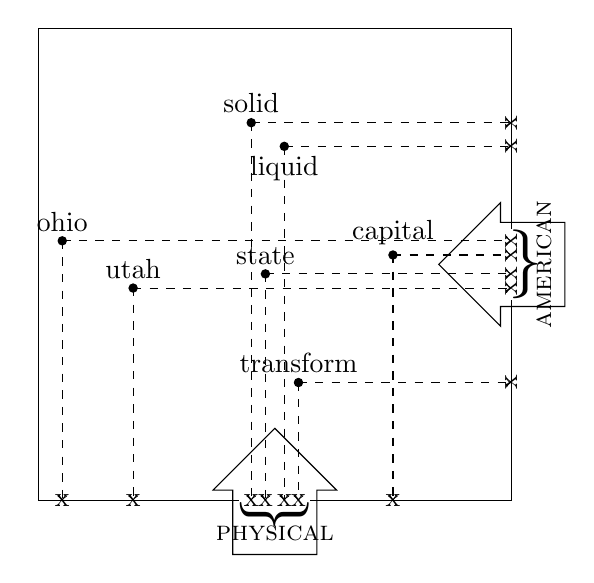
\begin{tikzpicture}[scale=0.06,baseline]
    	\draw (0,0)--(-100,0)--(-100,-100)--(-57.5,-100);
        \draw (-42.5,-100)--(0,-100)--(0,-57.5);
        \draw (0,-42.5)--(0,0);

    	\draw (-52,-52) [above] node {state};
        \fill (-52,-52) circle[radius=1];
        \draw[dashed,->] (-52,-52)--(-52,-100);
        \draw (-52,-100) node {x};
        \draw[dashed,->] (-52,-52)--(0,-52);
        \draw (0,-52) node [rotate=90] {x};

    	\draw (-55,-20) [above] node {solid};
        \fill (-55,-20) circle[radius=1];
        \draw[dashed,->] (-55,-20)--(-55,-100);
        \draw (-55,-100) node {x};
        \draw[dashed,->] (-55,-20)--(0,-20);
        \draw (0,-20) node [rotate=90] {x};

    	\draw (-25,-48) [above] node {capital};
        \fill (-25,-48) circle[radius=1];
        \draw[dashed,->] (-25,-48)--(-25,-100);
        \draw (-25,-100) node {x};
        \draw[dashed,->] (-25,-48)--(0,-48);
        \draw (0,-48) node [rotate=90] {x};

    	\draw (-48,-25) [below] node {liquid};
        \fill (-48,-25) circle[radius=1];
        \draw[dashed,->] (-48,-25)--(-48,-100);
        \draw (-48,-100) node {x};
        \draw[dashed,->] (-48,-25)--(0,-25);
        \draw (0,-25) node [rotate=90] {x};
        
        \draw (-45,-75) [above] node {transform};
        \fill (-45,-75) circle[radius=1];
        \draw [dashed,->] (-45,-75)--(-45,-100);
        \draw (-45,-100) node {x};
        \draw [dashed,->] (-45,-75)--(0,-75);
        \draw (0,-75) node [rotate=90] {x};
        
        \draw (-80,-55) [above] node {utah};
        \fill (-80,-55) circle[radius=1];
        \draw [dashed,->] (-80,-55)--(-80,-100);
        \draw (-80,-100) node {x};
        \draw [dashed,->] (-80,-55)--(0,-55);
        \draw (0,-55) node [rotate=90] {x};
        
        \draw (-95,-45) [above] node {ohio};
        \fill (-95,-45) circle[radius=1];
        \draw [dashed,->] (-95,-45)--(-95,-100);
        \draw (-95,-100) node {x};
        \draw [dashed,->] (-95,-45)--(0,-45);
        \draw (0,-45) node [rotate=90] {x};
        
        \node at (3,-50) {\Huge\}};
        \node at (-50,-103) [rotate=-90] {\Huge\}};
%        \node at (-50,-103) [rotate=-90] {\fontsize{80pt}{4em}\selectfont \}};
        
        \node at (-50,-102.5) [single arrow,draw,rotate=90,minimum height=40,minimum width=40,inner sep=15] {};
        \node at (-50,-107) {\textsc{physical}};
        \node at (2.5,-50) [single arrow,draw,rotate=180,,minimum height=40,minimum width=40,inner sep=15] {};
        \node at (7,-50) [rotate=90] {\textsc{american}};
    \end{tikzpicture}
    \end{subfigure}
    \caption{An ambiguous two-dimensional space of words relating to the term \emph{cat} (a), and a refined space where, based on two different one-dimensional projections, two different conceptual mappings of \emph{cat} emerge as word clusters (b).}
\end{figure}

\section{A Literal, Dynamic Language Model}

The model described here is characterised by two crucial features:

\begin{enumerate}
\item The dimensional features of the space are literally interpretable, in that they correspond to information theoretical statistics about the co-occurrence of words in a large scale corpus.
\item Following on this first point, the model operates by a procedure of continuously unfolding projections of subspaces, with the character of these projections determined by a continuous dimensional analysis based on input terms.
\end{enumerate}

In the first instance, the maintenance of dimensions populated by statistics pulled directly from a corpus traversal differentiates this approach from recent work by the likes of \cite{MikolovEA2013b} and \cite{PenningtonEA2014}, who have made use of neural networks and matrix factorisation to build models which perform well on hand-crafted test sets designed to test the models' performance on specific aspects of conceptualisation.  It is precisely the statistically concrete nature of the present model which allows it to remain conceptually dynamic.  Because the model's dimensions correspond literally to co-occurrence terms, an analysis of the dimensions that contribute strongly to terms observed as occurring in a particular contextual context can be drawn out and used to project a subspace from a base model.

\section{The Geometry of Metaphor}
The contextual dynamism of concepts is implicit in the isomorphic mappings between conceptual schemes at the root of \citepos{Lakoff} conceptual metaphors.  It is the internal anatomy of each conceptual scheme, produced by the environmental and consequent cultural entanglements inherent in language, that allows the alignment of conceptual schemes: there is always an implicit geometric foundation to these mappings (and this foundation is often rather more explicit, as in the case of, for example, orientation and conduit metaphors).  This project seeks to realise a practical implementation of this theoretical stance, in particular by utilising the geometric qualities of the contextualised subspaces that have already been described.  In particular, the al

There is once again a point of comparison with the models that have been described in the contemporary NLP literature here.  The analogy completions performed by the model of, for instance, \cite{MikolovEA2013b} employ a clever layer of basic linear algebra to word-vectors derived through the complex non-linear processing of corpus data.  These operations are, however, dependent on a certain consistency of scale within a space.  The algebraic relationship $\overrightarrow{king}-\overrightarrow{queen} = \overrightarrow{man}-\overrightarrow{woman}$, for instance, which has been discussed extensively in recent papers, depends on a comparability not only in terms of orientation but also in terms of distance between the spaces of \textsc{royals} and \textsc{people}.  This is a special category of analogy within a distributional model, however, as there are demonstrably comparable conceptualisations mappable from word clusterings of various scales.

By instead relying on the general geometric property of congruity rather than the specific scale of a space, the model described here offers a more robust approach to drawing connections between spaces.  If a concept is represented as a cluster of words that emerge in a distributional semantic subspace, then the theory here is that there should be mappings between the words in two different such subspaces which, taken as a whole, substantiate a conceptual metaphor.  The intuition here can be related to a more traditional transference view of metaphor: there will be some notable overlap between the co-occurrence profiles of the respective distributional spaces of, for instance, \textsc{surgery} and \textsc{butchery}.  By identifying this overlap, it should be possible to draw out correspondences between conceptual components such as \emph{scalpel} and \emph{cleaver}, and this in turn allows for the postulation of an alignment between the spaces which represents a metaphor.  Thus it is the geometry of the spaces which ultimately affords the opportunity for constructing a new semantic connection between conceptual domains, and the evident transference of intensions might be interpreted as an \emph{a posteriori} logical artefact of this process.

\begin{figure}
	\centering
	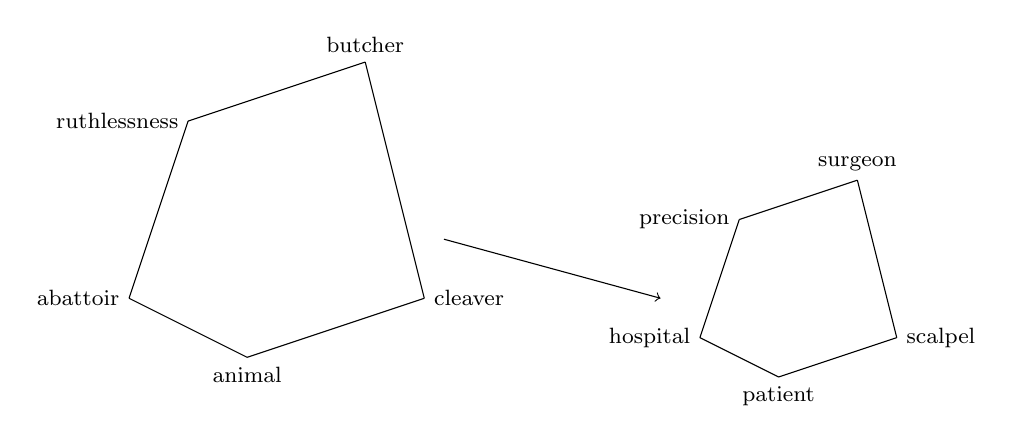
\begin{tikzpicture}[scale=0.25]
		\draw (6,15)--(15,18) node [above] {\footnotesize butcher};
		\draw (15,18)--(18,6) node [right] {\footnotesize cleaver};
		\draw (18,6)--(9,3) node [below] {\footnotesize animal};
		\draw (9,3)--(3,6)node [left] {\footnotesize abattoir};
		\draw (3,6)--(6,15) node [left] {\footnotesize ruthlessness};
		
		\draw [->] (19,9)--(30,6);
		
		\draw (34,10)--(40,12) node [above] {\footnotesize surgeon};
		\draw (40,12)--(42,4) node [right] {\footnotesize scalpel};
		\draw (42,4)--(36,2) node [below] {\footnotesize patient};
		\draw (36,2)--(32,4) node [left] {\footnotesize hospital};
		\draw (32,4)--(34,10) node [left] {\footnotesize precision};
	\end{tikzpicture}
	\caption{Congruences discovered in subregions of a vector space model suggest metaphoric mappings.  The regions do not necessarily have to be of the same scale in order to identify a possible alignment.}
\end{figure}

\chapter{Methodology}

\section{A Lexical Base Model}
The general model is trained by a single traversal of a large scale corpus.  Token by token, co-occurrence frequencies are tabulated for each word type, and the dimensions of the model are populated with information theoretical statistics measuring the mutual information associated with the observation of a context word occurring within a window of a certain number of words from a vocabulary word.  The result is a matrix with rows corresponding to word-vectors and columns corresponding to co-occurrence terms, such that an element $M_{w,c}$ measures the mutual information inherent in the co-occurrence of term $c$ with word $w$, where $N$ is the total count of word tokens in the corpus, $n_{w,c}$ is the frequency with which $c$ occurs in the context window of $w$, $n_w$ is the total frequency of word $w$, $n_c$ is the total count of times that $c$ is observed in the context of another word, and $a$ is a smoothing constant:

\begin{equation}\label{eq:MI}
M_{w,c} = \log_2 \left(\frac{n_{w,c} \times N}{n_w \times \left(n_c + a\right)} + 1\right)
\end{equation}

Once this base space is established, a dimensional analysis of input terms provides the basis for the projection of contextually informed subspaces.  So, for instance, given an input of terms $w_1$, $w_2$, and $w_3$, the model analyses the corresponding word-vectors $\overrightarrow{w_1}$, $\overrightarrow{w_2}$, and $\overrightarrow{w_3}$ to determine the salient co-occurrence dimensions shared between all three terms, which is to say, those universally non-zero dimensions with the highest mean value.  These dimensions are then used as the basis for the generation of a subspace, with the expectation that conceptually relevant terms will emerge in this new, significantly lower-dimensional space.  In particular, conceptual constituents are identified by searching for word-vectors that cluster around a positive central point considerably removed from the origin, by searching for the word-vectors with the greatest norms, and by searching for the word-vectors that are, on average, furthest away in terms of Euclidean distance from any other word vectors.

\section{Taxonomy Recapitulation}
The conceptual projections of the lexical base model perform particularly well at extending the membership of short lists of words corresponding to constituents of some conceptual category (so, for instance, a list containing \emph{lion}, \emph{tiger}, and \emph{bear} is expanded to include other exemplars of the concept \textsc{wild animal}).  With this in mind, a mechanism for establishing hypernymic relationships between such lists and terms denoting a general categorisation of such lists should lead to the effective reconstruction of hand-crafted lexical ontologies such as WordNet.

The proposed way forward at the time of writing is to establish a technique for analysing the co-occurrence data for singular terms and then to generate short lists of other words as candidates for list expansion operations.  This will most likely involve inspecting potential groupings of the terms that emerge from a subspace for high degrees of mutual co-occurrence, and then expanding top scoring sets to discover potential groupings of terms to be considered as constituents of a certain conceptual subtree.  There will also have to be a system for maintaining and then eventually comparing hypotheses about the conceptual relationships between the denotations of word pairs, as well as a mechanism for ultimately resolving these hypotheses into a well formed ontology.

\section{Analogy Completion}
Where work from researchers such as \cite{Mikolov}, \cite{Pennington}, and \cite{Levy} has focused on building distributional semantic spaces where simple arithmetical operations between word-vectors yield good results for certain types of analogies, the project presented here will focus on more robustly geometric methods to identify congruences between different contextualised projections.  As a first pass at this problem, searching for word-vectors that complete basic geometric transformations within a space seems like a viable approach to this task.  So, for instance, there is some transformation from the space of \textsc{butchery} to the space of \textsc{surgery} that preserves the overlapping co-occurrence relationships between words like \emph{cleaver} and \emph{scalpel} while aligning the 

\section{Metaphor Generation}
The ultimate goal of metaphor generation will involve a kind of reverse engineering of the model's approach to analogy completion: once the mechanism for performing analogical transformations between conceptually rooted word-subspaces has been refined, these transformations can be applied to a given projection based on the dimensional information inherent in the influence of some contextualising term.  Once these transformations are applied, the relatively sparse transformed source space can be searched for the points that best align with the geometry of the target space.

\chapter{Implementation and Results}
The base model has been trained on the English language text of Wikipedia, compiling statistics for a vocabulary of the 200,000 most frequent word types in the corpus and the terms that occur within a window of five words on either side of each token of the elements of the vocabulary.  In the cases presented here, the 200 most salient dimensions for each input query are used to project the contextualised subspaces.

\section{The Base Model and Projections}
Tests performed so far on the base model have returned good results for some sample contextual projections from the base model.  Two different types of input queries have been considered, one involving terms which together denote some contextually specific concept and another which offers a short list of conceptual exemplars.  Results for four sample queries are offered in~\ref{tab:context}, with the top ten output words in terms of norm being reported.

\begin{center}
	\begin{table}[h]\small
	\caption{Contextualised Word Spaces}
	\label{tab:context}
	\centering
	\begin{tabular}{|l|l|l|l|}
		\hline
		\multicolumn{2}{|c|}{\textsc{by hypernym}} & \multicolumn{2}{c|}{\textsc{by list}} \\
		\hline
		\multicolumn{1}{|c|}{\emph{wild animals}} & \multicolumn{1}{c|}{\emph{professional occupations}} & \multicolumn{1}{c|}{\emph{lion,tiger,bear}} & \multicolumn{1}{c|}{\emph{surgeon,butcher,builder}} \\
		\hline
		pocupines & technicians & leopard & bricklayer \\
		deer & accountants & dhole & grocer \\
		boar & technologists & hyena & apprenticed \\
		rabbits & therapists & boar & wheelwright \\
		foxes & electricians & langur & blacksmith \\
		raccoons & physiotherapists & macaque & plumber \\
		boars & dentists & tapir & shoemaker \\
		goats & hygienists & chital & industrialist \\
		squirrels & pharmacists & lion & joiner \\
		hares & nurses & rhinoceros & cabinetmaker \\
		\hline
	\end{tabular}
	\end{table}
\end{center}

\section{Taxonomies}
Some preliminary results, comparing the performance of the model described here versus the word2vec model of \cite{Mikolov}, are offered in~\ref{tab:hyper}.  The linear algebraic technique of using vector addition and then rating similar terms based on cosine similarity has been applied in the case of word2vec, as described in the literature.  Here \emph{hits} refer to terms that can be found in the WordNet subtree of terms associated with the appropriate synset for each input query, \emph{misses} refer to terms that are in WordNet but are not in the appropriate subtree, \emph{absent} tallies terms that are not in WordNet at all, and \emph{duplicate} indicates the count of terms that are morphemically identical to other words already returned by each model.

\begin{center}
	\begin{table}[h]\small
	\caption{Comparative Hypernymy}
	\label{tab:hyper}
	\centering
	\begin{tabular}{|r|l|l|l|l|}
		\cline{2-5}
		\multicolumn{1}{c|}{} & \multicolumn{2}{c|}{\emph{wild animals}} & \multicolumn{2}{c|}{\emph{visual artist}} \\
		\cline{2-5}
		\multicolumn{1}{c|}{} & \multicolumn{1}{c|}{\textsc{model}} & \multicolumn{1}{c|}{\textsc{w2v}} & \multicolumn{1}{c|}{\textsc{model}} & \multicolumn{1}{c|}{\textsc{w2v}} \\
		\hline
		\textsc{hits} & 40 & 34 & 16 & 8 \\
		\textsc{misses} & 5 & 9 & 24 & 30 \\
		\textsc{absent} & 2 & 2 & 7 & 9 \\
		\textsc{duplicate} & 3 & 5 & 3 & 3 \\
		\hline
	\end{tabular}
	\end{table}
\end{center}

\section{Analogies}
Preliminary experiments have been carried out to explore the comparative geometry of different word-spaces.  The approach thus far has been to measure the angles of the vertexes of different constellations of word-vectors within a subspace, and then to examine how these angles line up with the angles in another space with an eye towards describing a prospective conceptual mapping.  Experiments with the model's projections are under way, and results will be forthcoming.  For the time being, \ref{tab:metaphors} offers a comparison between terms within the general, non-reduced space.  Three mappings are offered; in each case, all possible alignments of words between each space are compared.  The average difference in angle between each of the two spaces for each possible alignment is calculated, and the ranking of the alignment that is deemed, for the purposes of this test run, conceptually satisfactory as compared to all other alignments is returned.  The high performance of the appropriate alignments even in the unrefined base space motivates further and more rigorous testing of mappings between projected spaces, which should remit a much higher degree of conceptual coherence.

\begin{table}[h]\footnotesize
\centering
\caption{Angular Mappings of Conceptual Regions}
\label{tab:metaphors}
	\begin{tabular}{|l||l|l|l|}
		\hline
		target & ROYALS & SURGERY & EMOTIONS \\
		source & PEOPLE & BUTCHERY & ORIENTATIONS \\
		\hline
		rank & 1 out of 24 & 15 out of 720 & 3 out of 720 \\
		mean & 0.062 & 0.046 & 0.048 \\
		high & - & 0.037 & 0.045 \\
		low & 0.198 & 0.094 & 0.101 \\
		\hline
		\multirow{6}{*}{mappings} & man $\rightarrow$ king & butcher $\rightarrow$ surgeon & up $\rightarrow$ happiness \\
			&woman $\rightarrow$ queen & cleaver $\rightarrow$ scalpel & down $\rightarrow$ sadness \\
			&boy $\rightarrow$ prince & abattoir $\rightarrow$ hospital & out $\rightarrow$ loneliness \\
			&girl $\rightarrow$ princess & lamb $\rightarrow$ patient & in $\rightarrow$ togetherness \\
			&& pig slaught. $\rightarrow$ operation & atop $\rightarrow$ control \\
			&& ruthlessness $\rightarrow$ precision & beneath $\rightarrow$ incapacity \\
		\hline
	\end{tabular}
\end{table}

\chapter{Evaluation}
This section for now very broadly outlines some of the evaluative objectives of this project.

but the crucial

considered here is the necessity of resorting to some real world mechanisms for assessing the model's performance, both through formal studies with human subjects and through a less structured but more public testing of the system 

\section{Taxonomy and Analogy}
One problem inherent in the use of datasets, be they test sets specifically designed to examine features of computational language models or general and highly public frameworks such as WordNet or DBpedia, is the necessarily biased and incomplete process of assigning conceptual relationships to senses of words.  As such, in addition to the straightforward analysis of results over test sets and reporting of precision, recall, and related statistics for ontology recapitulation, it will probably be necessary to resort to asking human subjects about the efficacy of the model's conceptual mappings.

\section{Metaphor}
Even more than with the only moderately controversial tasks of determining whether conceptual and analogical relationships are appropriately captured by the models output, the problem of assessing the creative value of metaphoric artefacts generated by the model is fraught with the 

In the end, the criteria of usefulness and novelty generally taken as the basic standard for computationally creative output can serve as a good guide for the model's target, but not as much more than this.  Simply asking humans whether they consider the model to be performing along these lines must be a hopelessly subjective enterprise

\chapter{Conclusion}


\bibliographystyle{apacite}
\bibliography{/home/masteradamo/academy/Cite.bib}

% Start the appendix (inc. author's publications)
\begin{appendix}
%\chapter{Author's publications}

% publications goes here

\subsection*{Journal papers}
\begin{enumerate}
  \item \textbf{Y. Gao}, X. Chen, Z. Ying and C. G. Parini, ``Design and Performance
Investigation of a Dual-element PIFA Array at 2.5 GHz for MIMO Terminals," \emph{IEEE Trans. on
Antennas and Propagation}. (Revising)

\end{enumerate}


\subsection*{Conference papers}


\begin{enumerate}
  \item \textbf{Y. Gao}, X. Chen, Z. Ying and C. G. Parini , ``Further Investigation of a
Dual-Element Diversity PIFA for MIMO Applications at 2.5 GHz Band," \emph{IEEE International
Symposium on Antennas and Propagation (AP-S)} , Honolulu, Hawaii, USA  June, 2007. (Accepted)
    
\end{enumerate}

\subsection*{Project report}
\begin{enumerate}
  \item X. Chen and \textbf{Y. Gao}, ``Final Report on Modelling of Difficult Environments,"
  Galileo Advance Concept project final report (GAC/EUT/DT/219), 9th June - 31 October 2007.
  
\end{enumerate}



\renewcommand{\thefigure}{B.\arabic{figure}}
\chapter{Solutions for the Examples in Chapter 2}
\label{examples_solutions}
\section{Example 1: Antenna Spacing Effect}

\textbf{Step 1:} Get the $H_{norm}H_{norm}^\dagger$, set $2{\pi}R/\lambda={\omega}_1$ and
$2{\pi}(\overline{R})/\lambda={\omega}_2$ ($\lambda$ is the wavelength), so
\begin{equation}
H_{norm} = \frac{1}{\sqrt 2 }\left( {{\begin{array}{*{20}c}
 {e^{ - j\omega _1 }} \hfill & {e^{ - j\omega _2 }} \hfill \\
 {e^{ - j\omega _2 }} \hfill & {e^{ - j\omega _1 }} \hfill \\
\end{array} }} \right)
\end{equation}
Note: $H_{norm}^\dagger=(\overline{H_{norm}})^T$ and $e^{j\theta}=cos\theta +jsin\theta$
\begin{equation}
\begin{array}{l}
 H_{norm}H_{norm}^\dagger = \frac{1}{2}\left( {{\begin{array}{*{20}c}
 {e^{ - j\omega _1 }} \hfill & {e^{ - j\omega _2 }} \hfill \\
 {e^{ - j\omega _2 }} \hfill & {e^{ - j\omega _1 }} \hfill \\
\end{array} }} \right)\left( {{\begin{array}{*{20}c}
 {e^{j\omega _1 }} \hfill & {e^{j\omega _2 }} \hfill \\
 {e^{j\omega _2 }} \hfill & {e^{j\omega _1 }} \hfill \\
\end{array} }} \right) \\
 = \frac{1}{2}\left( {{\begin{array}{*{20}c}
 {1 + 1} \hfill & {e^{ - j(\omega _1 - \omega _2 )} + e^{ - j(\omega _1 -
\omega _2 )}} \hfill \\
 {e^{ - j(\omega _1 - \omega _2 )} + e^{ - j(\omega _1 - \omega _2 )}}
\hfill & {1 + 1} \hfill \\
\end{array} }} \right) \\
 = \left( {{\begin{array}{*{20}c}
 1 \hfill & {\cos (\omega _1 - \omega _2 )} \hfill \\
 {\cos (\omega _1 - \omega _2 )} \hfill & 1 \hfill \\
\end{array} }} \right) \\
 \end{array}
\end{equation}
\textbf{Step 2:} Get the eigenvalue of $H_{norm}H_{norm}^\dagger$, here set $\lambda$ as
eigenvalue, then,
\begin{equation}
\left( {{\begin{array}{*{20}c}
 {1 - \lambda } \hfill & {\cos (\omega _1 - \omega _2 )} \hfill \\
 {\cos (\omega _1 - \omega _2 )} \hfill & {1 - \lambda } \hfill \\
\end{array} }} \right) = 0
\end{equation}
and $\omega_1-\omega_2=2{\pi}R/\lambda-2{\pi}(\overline{R})/\lambda=-54^o$, so
$\lambda=1{\pm}cos(\omega_1-\omega_2){\approx}1{\pm}0.59$. Hence, $\lambda_1=1.59$ and
$\lambda_2=0.41$.





\end{appendix}

\end{document}
% That's all of it!
